% Graph: Análise do volume de dados no Experimento Gamma
\begin{figure}[H]
	\centering
	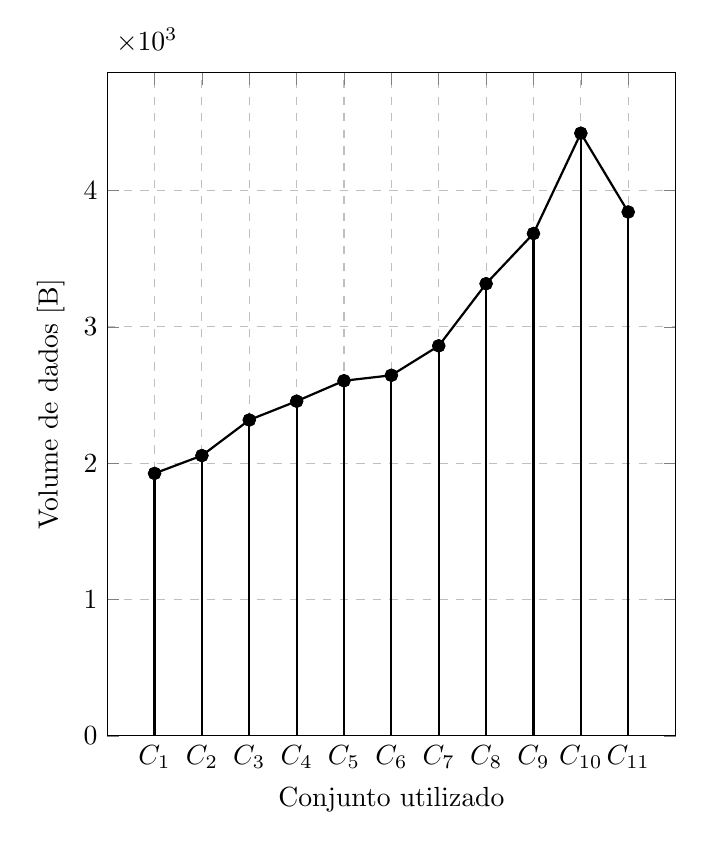
\begin{tikzpicture}
		\begin{axis}[
			% title={Análise de volume de dados},
			symbolic x coords={$C_1$, $C_2$, $C_3$, $C_4$, $C_5$, $C_6$, $C_7$, $C_8$, $C_9$, $C_{10}$, $C_{11}$},
			xtick={$C_1$, $C_2$, $C_3$, $C_4$, $C_5$, $C_6$, $C_7$, $C_8$, $C_9$, $C_{10}$, $C_{11}$},
			ylabel={Volume de dados [B]},
			xlabel={Conjunto utilizado},
			ymin=0,
			bar width=10pt,
			ymajorgrids=true,
			xmajorgrids=true,
			grid style=dashed,
			height=10cm,
			width=8.8cm,
			tick scale binop=\times,
			scaled y ticks=base 10:-3,
		]
		 
		\addplot[color=black, solid, thick, ycomb, mark=*]
			coordinates {
				($C_1$,1925)
				($C_2$,2056)
				($C_3$,2317)
				($C_4$,2455)
				($C_5$,2605)
				($C_6$,2645)
				($C_7$,2861)
				($C_8$,3317)
				($C_9$,3685)
				($C_{10}$,4421)
				($C_{11}$,3843)
			};
			
			\addplot[color=black, solid, thick, mark=*]
			coordinates {
				($C_1$,1925)
				($C_2$,2056)
				($C_3$,2317)
				($C_4$,2455)
				($C_5$,2605)
				($C_6$,2645)
				($C_7$,2861)
				($C_8$,3317)
				($C_9$,3685)
				($C_{10}$,4421)
				($C_{11}$,3843)
			};

		\end{axis}
	\end{tikzpicture}
	\caption{Análise de volume de dados.}
	\label{graph:dataVolResultsGamma}
\end{figure}